\section{Algorytm}

Filtr Savitzky-Golay pozwala wygładzić cyfrowy sygnał. Jego działanie opiera się na lokalnym przybliżeniu próbek sygnału wielomianami niskiego rzędu \cite{whatissg}.

Mając dany sygnał x[n], poszukujemy wielomianu
\begin{equation}
p(n) = \sum\limits_{k=0}^N a_k n^k
\end{equation}
który w otoczeniu $2M+1$ punktów minimalizuje kwadrat błędu aproksymacji
\begin{equation}
\epsilon_N = \sum\limits_{n=-M}^M (p(n) - x[n])^2
\end{equation}

Wtedy dla próbki centralnej pośród $2M+1$ punktów (ma ona indeks $n=0$) wartość odfiltrowanego sygnału przyjmuje
\begin{equation}
y[0] = p(0) = a_0
\end{equation}

W praktyce filtr Savitzky-Golay realizuje swoje zadanie obliczając splot kilku aktualnie branych pod uwagę punktów z wielomianową aproksymacją ciągu z jednostkowym impulsem w środku sekwencji.
\begin{equation}
y[n] = \sum\limits_{m=n-M}^{n+M} h[n-m] x[m]
\end{equation}
gdzie $h$ jest wynikiem interpolacji wielomianem stopnia $N$ sekwencji z jednostkowym impulsem, np. $[0, 0, 0, 1, 0, 0, 0]$ dla $M=3$.


\newpage
\section{Prototyp programu}
\subsection{Użyte moduły}
Przed przystąpieniem do pracy nad algorytmem, użyliśmy biblioteki \textbf{WFDB} dla środowiska MATLAB, która umożliwiła pobranie danych EKG z bazy MIT-BIH\cite{mit-bih}.

W prototypowej wersji programu użyliśmy modułu \textbf{NumPy} do operacji na macierzach i operacji numerycznych, w tym: interpolacji wielomianowej, sklejania i obracania wektorów. 
Moduł matplotlib.pyplot posłużył do obrazowania wyników.

\subsection{Oprogramowanie algorytmu}
Ponieważ odpowiedź impulsowa filtru $h$ jest niezależna od wartości sygnału, wartości wektora $h$ o długości $2m+1$ wystarczy obliczyć raz, a następnie obliczyć wartość konwolucji sygnału z taką maską. Wartości maski zostały pokazane na rysunku \ref{rys:impuls}.

\begin{figure}[!htb]
  \begin{center}
    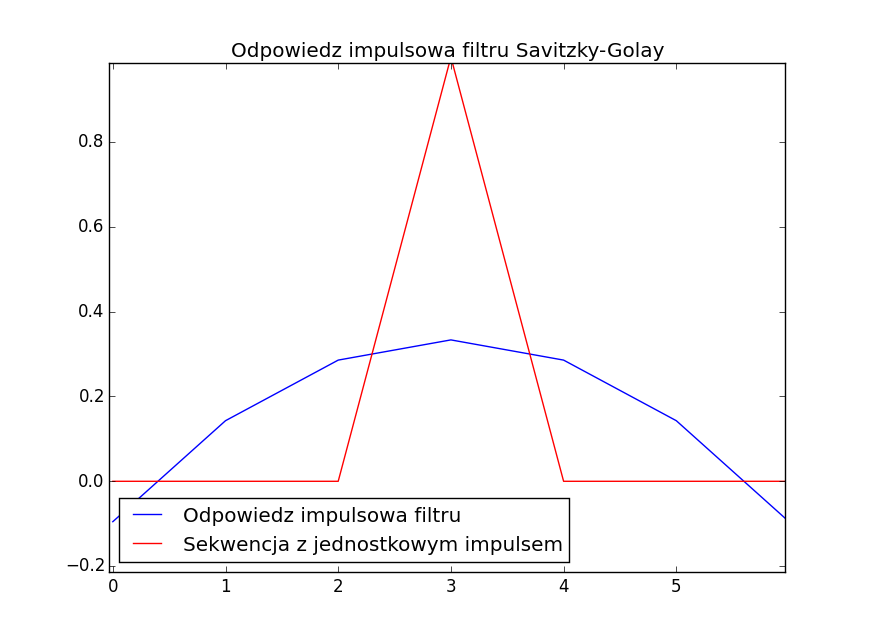
\includegraphics[scale=0.8]
    {img/impulse.png}
  \end{center}
  \caption{Odpowiedź impulsowa filtru, uzyskana jako interpolacja wielomianem $N=2$ stopnia serii $2M+1=7$ próbek z jednostkowym impulsem pośrodku}
  \label{rys:impuls}
\end{figure}

\subsection{Wartości brzegowe}
Algorytm w każdym punkcie potrzebuje do obliczeń $M$ punktów z lewej i $M$ punktów z prawej strony, zatem należy zdecydować o zachowaniu programu na początku i na końcu spróbkowanego sygnału.

Istnieje kilka możliwych rozwiązań:
\begin{enumerate}
\item Zawijanie - algorytm wykorzysta pierwsze $M$ punktów na końcu oraz ostatnie $M$ punktów na początku sygnału
\item Odbicie - na brzegach zostaną wykorzystane najbliższe punkty, jednak w odwróconej kolejności
\item Użycie stałej, ustalonej wartości
\item Najbliższy sąsiad - poza granicami sygnału zostaną dopisane punkty równe pierwszej próbce (na początku) i ostatniej próbce (na końcu)
\end{enumerate}

W prototypie wybraliśmy rozwiązanie 2. Jeśli ostatnie punkty mają wartości $[6, 7, 8, 9]$, to dopisane poza prawą granicą punkty otrzymają wartości $[8, 7, 6]$.


Przebieg filtracji uzyskanej za pomocą prototypu Python przedstawia wykres \ref{rys:savitzky_py}

\begin{figure}[!htb]
  \begin{center}
    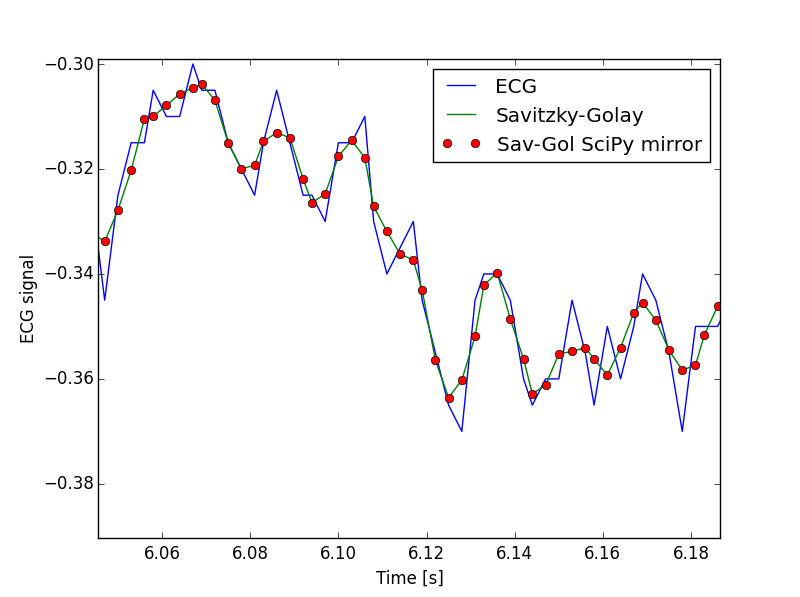
\includegraphics[scale=0.8]
    {img/prototype.png}
  \end{center}
  \caption{Wygładzanie metodą Savitzky-Golay z oknem 7 próbek (M=3) i aproksymacją wielomianem N=2 stopnia. Porównanie prototypu z funkcją z modułu SciPy.signals}
  \label{rys:savitzky_py}
\end{figure}

Aktualny kod dostępny w repozytorium https://github.com/Qbicz/Savitzky-Golay


